\acao{Ação 3.2.2.3 – Implantação e reabilitação dos sistemas coletivos de abastecimento de água}

\phantomsection
\addcontentsline{toc}{subsection}{1. Contextualização}
\subsection*{1. Contextualização}

A ação implanta ou reabilita 83 sistemas coletivos de abastecimento de água em comunidades rurais, com captação subterrânea por poço tubular profundo, desinfecção por cloração, reservação, rede de distribuição e ligações domiciliares com hidrômetro. Os sistemas atendem 5.810 domicílios, cerca de 16,3 mil pessoas, entre 2028 e 2033 (PARANÁ, 2026; IAT, 2026a).

No meio rural do Paraná, 99,59\% dos domicílios dispõem de água canalizada, segundo o Censo 2022, mas apenas 16,92\% do abastecimento provém de sistemas coletivos com tratamento completo (IAT, 2026a). Predominam nascentes e poços rasos escavados (cacimbas), em grande parte contaminados por agrotóxicos, metais e coliformes e sujeitos à redução de vazão nas estiagens recorrentes no Estado. O consumo de água contaminada está associado a doenças de veiculação hídrica, como diarreia, hepatite e esquistossomose.

Por essas razões, a ação adota a captação de água subterrânea por poço tubular profundo. A água subterrânea apresenta, em geral, melhor qualidade microbiológica e menor sensibilidade à variabilidade climática, o que, na maior parte dos casos, restringe o tratamento à desinfecção por cloração. A captação subterrânea tem também menor custo, menor prazo de implantação e menor impacto ambiental que a captação superficial, que requer barragem, adutora e estação de tratamento (IAT, 2026a).

A Figura~\ref{esquema-saa} apresenta os componentes de um sistema típico.

\begin{figure}[H]
  \centering
  \caption{Componentes de um sistema coletivo de abastecimento de água rural}\label{esquema-saa}
  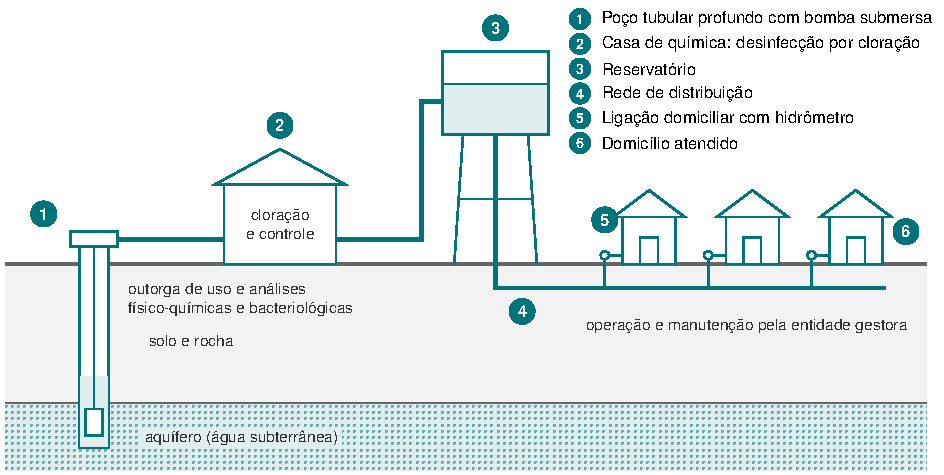
\includegraphics[width=15.98cm]{figuras/f-esquema-saa.pdf}
  \fonteMOP{Fonte: IAT (2026). Esquema ilustrativo, sem escala.}
  % Texto alternativo: Esquema em corte com poço tubular profundo, casa de química, reservatório elevado, rede de distribuição e domicílios com hidrômetro.
\end{figure}

A ação apoia-se na experiência do Programa Água no Campo, no qual o IAT perfura poços e implanta sistemas coletivos em comunidades não atendidas pelas companhias de saneamento. Desde 2019, o programa perfurou 801 poços, com investimento aproximado de R\$~12,3 milhões e cerca de 250 mil pessoas beneficiadas; no primeiro semestre de 2025, foram 39 poços em 21 municípios, para 1.253 famílias (IAT, 2026a). Os resultados esperados incluem a redução das doenças de veiculação hídrica e dos gastos públicos com saúde, a melhoria das condições de vida, o estímulo à permanência das famílias no campo e o fortalecimento da organização comunitária.

A ação constitui a principal contribuição do IAT ao indicador de pessoas atendidas com água gerida de forma segura: cerca de 16,3 mil das 59.780 pessoas previstas. As demais decorrem do Programa Sanepar Rural.

\textbf{Inclui:} estudos preliminares e regularização das áreas; locação, perfuração, teste de vazão, análises físico-químicas e bacteriológicas e outorga dos poços; projetos básico e executivo; licenciamento ambiental; obras da casa de química, do reservatório, das instalações eletromecânicas, da rede e das ligações com hidrômetro; reabilitação de sistemas existentes operados por associações; pré-operação, testes e capacitação dos operadores; e entrega à entidade gestora.

\textbf{Não inclui:} a supervisão independente das obras, o modelo de gestão, o trabalho técnico-social, o esgotamento sanitário e os sistemas do Programa Sanepar Rural, objeto de ações próprias.

\textbf{Valor previsto:} R\$~107,90 milhões (empréstimo BIRD: R\$~107,90 milhões; contrapartida: R\$~0,00 milhões), conforme a planilha PSH\_CUSTO\_Consolidada.

\phantomsection
\addcontentsline{toc}{subsection}{2. Área de atuação}
\subsection*{2. Área de atuação}

A ação abrange todo o Estado, nas Microrregiões de Água e Esgoto, e restringe-se às comunidades que atendem aos critérios de seleção (Figura~\ref{selecao-comunidades}). O primeiro critério é o adensamento: comunidade ou conjunto de comunidades com 70 ou mais domicílios ocupados, número mínimo que viabiliza o modelo de gestão.

O segundo critério é o desempenho do município no IPDM, que varia de 0 a 1 e classifica os municípios em quatro estratos: baixo (0 a menos de 0,4), médio baixo (0,4 a menos de 0,6), médio (0,6 a menos de 0,8) e alto (0,8 a 1,0). A ação restringe-se aos municípios de médio baixo e de médio desempenho.

Consideram-se, ainda, as solicitações de perfuração de poços já encaminhadas pelos municípios ao IAT e a existência de associações de moradores que operam sistemas com necessidade de complementação ou melhoria. Por fim, a comunidade somente prossegue para a implantação na ausência de impedimentos à perfuração: disponibilidade hídrica insuficiente no aquífero, condições geológicas que inviabilizem a obra, falhas geológicas com risco de contaminação ou de interrupção do fluxo, contaminantes que comprometam a potabilidade ou restrições legais e ambientais (IAT, 2026a).

\begin{figure}[H]
  \centering
  \caption{Critérios de seleção das comunidades atendidas com água}\label{selecao-comunidades}
  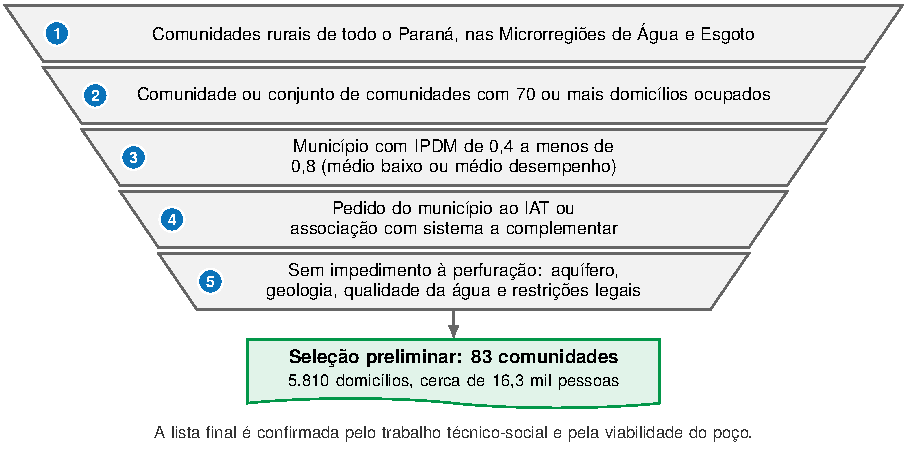
\includegraphics[width=15.37cm]{figuras/f-selecao-comunidades.pdf}
  \fonteMOP{Fonte: IAT (2026), com base em IAT (2026a).}
  % Texto alternativo: Funil com os cinco critérios de seleção das comunidades, que resulta na seleção preliminar de 83 comunidades e 5.810 domicílios.
\end{figure}

\pendencia{Justificar a exclusão dos municípios de baixo e de alto desempenho no IPDM. O Banco Mundial costuma questionar a exclusão de municípios mais vulneráveis.}

A aplicação preliminar dos critérios indicou 83 comunidades, com 5.810 domicílios, considerada a média de 70 domicílios por comunidade e de 2,8 habitantes por domicílio (Censo 2022). As áreas de maior concentração de domicílios rurais e os municípios consorciados ao CISPAR constam da Figura~\ref{mapa}. A lista final é confirmada pelo trabalho técnico-social e pela viabilidade do poço (Etapa 2).

\pendencia{O Acordo de Empréstimo, item (j)(vii) das definições, exige a identificação das áreas rurais da Parte 3.2. Anexar a lista das 83 comunidades selecionadas, com município e coordenadas, ou o mapa com a respectiva localização.}

\phantomsection
\addcontentsline{toc}{subsection}{3. Arranjo institucional e partes interessadas}
\subsection*{3. Arranjo institucional e partes interessadas}

A ação é coordenada pelo IAT, por meio da DISAR, responsável pelo planejamento, pela contratação, pela fiscalização e pelo recebimento dos sistemas. No próprio IAT, a Diretoria de Licenciamento e Outorga emite a outorga de direito de uso de recursos hídricos e as licenças ambientais. As prefeituras apoiam a regularização das áreas e a articulação local, a entidade gestora recebe e opera cada sistema, e a UGP acompanha a execução e consolida o reporte ao Banco Mundial.

\begin{itemize}
  \item \textbf{Coexecutora:} SEAB, na implementação local junto às comunidades;
  \item \textbf{Intervenientes:} prefeituras; entidades gestoras; empresas contratadas para projetos e obras; laboratórios contratados para as análises de potabilidade; empresa supervisora das obras;
  \item \textbf{Público envolvido:} proprietários das áreas do poço, do reservatório e da rede; moradores das comunidades.
\end{itemize}

\pendencia{O MOP de março e a nota técnica preveem a participação da instituição parceira da área rural na implementação local, sem detalhar o seu papel nesta ação. Detalhar a atuação da SEAB.}

Os beneficiários diretos são os moradores dos 5.810 domicílios ligados aos sistemas, cerca de 16,3 mil pessoas, selecionados pelos critérios do item 2. Os beneficiários indiretos são os municípios, com a redução de gastos com saúde, e a população do entorno, que deixa de depender de fontes contaminadas.

\phantomsection
\addcontentsline{toc}{subsection}{4. Processo de execução operacional}
\subsection*{4. Processo de execução operacional}

A implantação de cada sistema compreende seis etapas (Figura~\ref{raias-3223}). Duas premissas aplicam-se a todas: as comunidades atendidas são confirmadas pelo trabalho técnico-social, e o modelo de gestão é pactuado antes das obras. O produto final de cada sistema é o Termo de Recebimento Definitivo (TRD), emitido pelo IAT após o aceite da entidade gestora.

\begin{figure}[H]
  \centering
  \caption{Fluxograma da implantação dos sistemas coletivos de abastecimento de água: entradas, etapas por responsável e saídas}\label{raias-3223}
  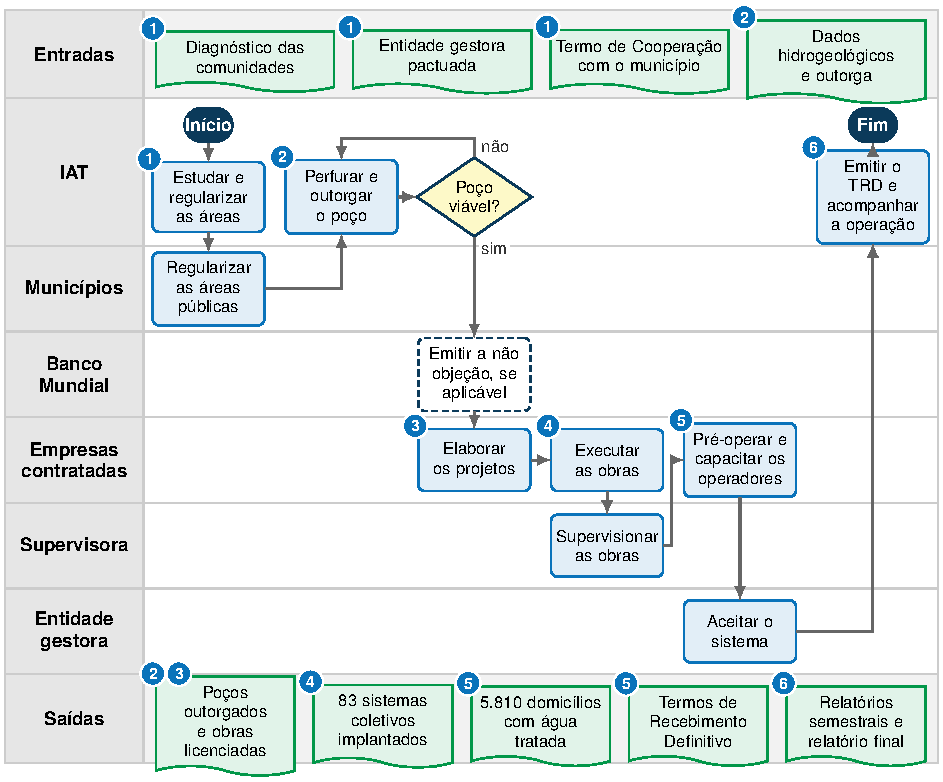
\includegraphics[width=15.96cm]{figuras/g-raias-3223.pdf}
  \fonteMOP{Fonte: IAT (2026).}
  % Texto alternativo: Fluxograma em raias da implantação dos sistemas coletivos de abastecimento de água, com uma raia por instituição, as etapas numeradas na raia do executor, as entradas no topo e as saídas na base.
\end{figure}

\phantomsection
\subsubsection*{4.1 Etapa 1: Estudos preliminares e regularização das áreas}

\textbf{Atividades:} estudos de viabilidade técnica, social e ambiental; levantamento de campo geológico e hidrogeológico; verificação da titularidade e da situação fundiária das áreas do poço, do reservatório e das demais estruturas; formalização da doação, da cessão ou da servidão das áreas, com anuência do proprietário; anteprojeto e investigação social. A Figura~\ref{captacao} apresenta a sequência das Etapas 1 a 3.

\begin{figure}[H]
  \centering
  \caption{Captação subterrânea, projeto e licenciamento (Etapas 1 a 3)}\label{captacao}
  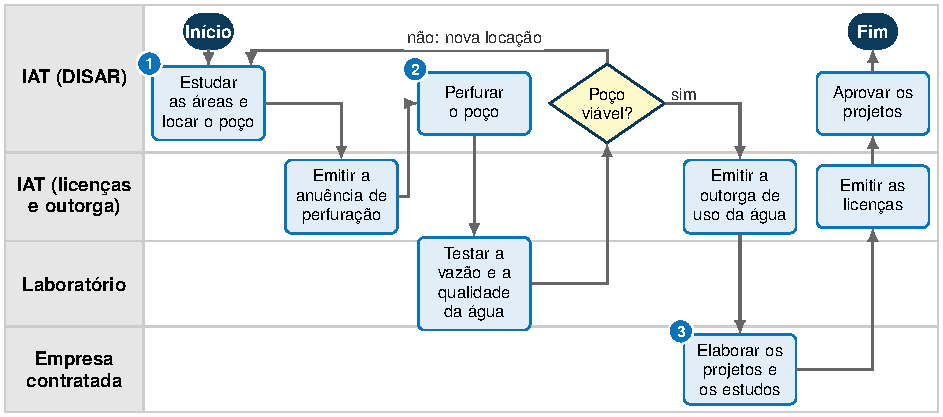
\includegraphics[width=15.96cm]{figuras/f-captacao.pdf}
  \fonteMOP{Fonte: IAT (2026), com base em IAT (2026b).}
  % Texto alternativo: Fluxograma em raias da DISAR, da área de licenciamento e outorga do IAT, do laboratório e da empresa contratada, com a decisão sobre a viabilidade do poço.
\end{figure}

\textbf{Entradas:} diagnóstico da comunidade (trabalho técnico-social); entidade gestora pactuada; Termo de Cooperação.

\textbf{Responsáveis:} IAT (executa e aprova); prefeituras (executam a regularização das áreas públicas); proprietários (consultados).

\textbf{Produto:} áreas regularizadas e anteprojeto aprovado.

\phantomsection
\subsubsection*{4.2 Etapa 2: Perfuração e outorga do poço}

\textbf{Atividades:} locação do poço e projeto construtivo; anuência prévia de perfuração; perfuração conforme as normas técnicas de projeto e construção de poços; teste de vazão; análises físico-químicas e bacteriológicas da água; outorga de direito de uso. Em caso de vazão ou qualidade insuficientes, o IAT procede a nova locação ou substitui a comunidade por outra que atenda aos critérios. O IAT dispõe de equipes próprias de perfuração, com equipamentos e equipe técnica para mais de 150 poços por ano (IAT, 2026a).

\textbf{Entradas:} áreas regularizadas; estudo hidrogeológico.

\textbf{Responsáveis:} equipe de perfuração do IAT ou empresa contratada (executa); laboratório contratado (análises); IAT (aprova e emite a outorga).

\textbf{Produto:} poço perfurado, testado e outorgado.

\pendencia{A nota técnica prevê a perfuração dos poços pelas equipes do IAT; o MOP de março previa a contratação integrada do poço. Definir o responsável pela perfuração.}

\phantomsection
\subsubsection*{4.3 Etapa 3: Contratação integrada, projetos e licenças}

\textbf{Atividades:} contratação integrada, na qual a mesma empresa elabora os projetos executivos e executa as obras; projetos básico e executivo da casa de química, do reservatório, das instalações eletromecânicas, da rede e das ligações; aprovação dos projetos pelo IAT; estudos ambientais e sociais e obtenção das licenças. As obras iniciam-se somente após a emissão da outorga e das licenças.

\textbf{Entradas:} poço outorgado; vazão e qualidade da água; anteprojeto.

\textbf{Responsáveis:} IAT (contrata, aprova os projetos e emite as licenças); empresa contratada (elabora os projetos); Banco Mundial (consultado, quando houver revisão prévia).

\textbf{Produto:} projetos aprovados e licenças emitidas.

\pendencia{O MOP define “contratação integrada” como aquela em que o contratado elabora o projeto executivo e executa a obra, o que corresponde à contratação semi-integrada da Lei nº~14.133/2021 (art. 6º, XXXIII). Definir o regime e verificar a compatibilidade com o Regulamento de Aquisições do Banco Mundial.}

\phantomsection
\subsubsection*{4.4 Etapa 4: Execução das obras}

\textbf{Atividades:} a obra é acompanhada em três níveis (Figura~\ref{obras}): o executor constrói conforme o projeto e instala hidrômetro em cada ligação domiciliar; a supervisora acompanha a execução e registra o andamento em relatórios mensais; e a fiscalização do IAT verifica a conformidade com o projeto e as normas. Constatada não conformidade, o executor procede à correção, e a obra é submetida a nova verificação. Atestada a conformidade, o IAT emite o atesto de recebimento, acompanhado dos laudos de vistoria e do projeto \textit{as built}.

\begin{figure}[H]
  \centering
  \caption{Execução, supervisão e fiscalização das obras, por responsável}\label{obras}
  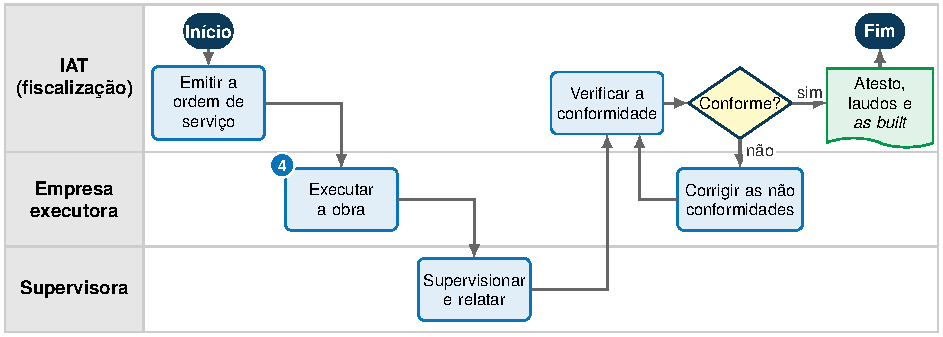
\includegraphics[width=15.96cm]{figuras/f-obras.pdf}
  \fonteMOP{Fonte: IAT (2026), com base em IAT (2026b).}
  % Texto alternativo: Fluxograma em raias da fiscalização do IAT, da empresa executora e da supervisora, com a decisão de conformidade e a correção das não conformidades.
\end{figure}

\textbf{Entradas:} projetos aprovados; outorga e licenças; ordem de serviço.

\textbf{Responsáveis:} empresa contratada (executa); supervisora (acompanha); IAT (fiscaliza e aprova); prefeituras (consultadas).

\textbf{Produto:} sistema implantado, com atesto de recebimento, laudos de vistoria e projeto \textit{as built}.

\pendencia{No MOP de março, a quantidade de hidrômetros consta como “XXX”. Pela meta de domicílios, são 5.810 hidrômetros, um por ligação; confirmar.}

\phantomsection
\subsubsection*{4.5 Etapa 5: Pré-operação, capacitação e entrega}

\textbf{Atividades:} pré-operação e testes de funcionamento; capacitação dos operadores locais, conforme o Plano de Operação e Manutenção; reunião técnica de entrega com a comunidade e a entidade gestora; aceite da entidade gestora; emissão do TRD (Figura~\ref{entrega}).

\begin{figure}[H]
  \centering
  \caption{Transferência, operação e encerramento dos sistemas de abastecimento}\label{entrega}
  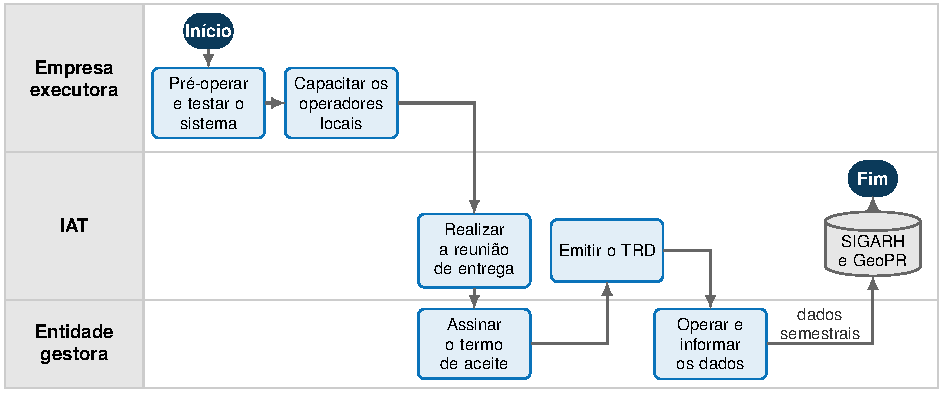
\includegraphics[width=15.96cm]{figuras/f-entrega.pdf}
  \fonteMOP{Fonte: IAT (2026), com base em IAT (2026b).}
  % Texto alternativo: Fluxograma em raias da empresa executora, do IAT e da entidade gestora, da pré-operação ao registro dos dados de operação no SIGARH e no GeoPR.
\end{figure}

\textbf{Entradas:} sistema implantado; entidade gestora constituída.

\textbf{Responsáveis:} empresa contratada (pré-operação e capacitação); entidade gestora (aceita o sistema); IAT (aprova e emite o TRD).

\textbf{Produto:} Termo de Recebimento Definitivo e operadores capacitados.

\phantomsection
\subsubsection*{4.6 Etapa 6: Acompanhamento pós-implantação e encerramento}

\textbf{Atividades:} suporte técnico pós-implantação; avaliação semestral de desempenho; acompanhamento da qualidade da água distribuída, conforme o padrão de potabilidade (BRASIL, 2021); registro dos dados no SIGARH e no GeoPR; relatório final e prestação de contas.

\textbf{Entradas:} TRD; dados de operação informados pela entidade gestora.

\textbf{Responsáveis:} IAT (executa); entidade gestora (informa os dados de operação); UGP (valida o relatório final).

\textbf{Produto:} relatórios semestrais de desempenho e relatório final.

\phantomsection
\subsubsection*{4.7 Modalidade de execução}

O item de custo é o de sistemas coletivos de abastecimento de água: 83 sistemas a R\$~1,3 milhão, no total de R\$~107,90 milhões, com recursos do empréstimo do BIRD. Os projetos executivos e as obras são contratados mediante licitação, em regime de contratação integrada, conforme o Caderno AQ; os ensaios laboratoriais de potabilidade também são licitados.

Os estudos preliminares, a regularização das áreas e a outorga são executados diretamente pelo IAT. A perfuração pode ser executada pelas equipes do IAT ou incluída na contratação das obras.

\pendencia{A nota técnica estima R\$~1,4 milhão por sistema; prevalece o valor da planilha de custos (R\$~1,3 milhão).}

\phantomsection
\addcontentsline{toc}{subsection}{5. Matriz de responsabilidades}
\subsection*{5. Matriz de responsabilidades}

O Quadro~\ref{raci-3223} apresenta o papel de cada parte em cada etapa.

\begin{quadro}[H]
  \caption{Matriz de responsabilidades da implantação dos sistemas coletivos de abastecimento de água}\label{raci-3223}
  \footnotesize\renewcommand{\arraystretch}{1.25}\setlength{\tabcolsep}{3pt}
  \begin{tabular}{>{\raggedright\arraybackslash}p{\dimexpr 0.2536\linewidth-2\tabcolsep\relax}>{\centering\arraybackslash}p{\dimexpr 0.0882\linewidth-2\tabcolsep\relax}>{\centering\arraybackslash}p{\dimexpr 0.0882\linewidth-2\tabcolsep\relax}>{\centering\arraybackslash}p{\dimexpr 0.0882\linewidth-2\tabcolsep\relax}>{\centering\arraybackslash}p{\dimexpr 0.0882\linewidth-2\tabcolsep\relax}>{\centering\arraybackslash}p{\dimexpr 0.0882\linewidth-2\tabcolsep\relax}>{\centering\arraybackslash}p{\dimexpr 0.0882\linewidth-2\tabcolsep\relax}>{\centering\arraybackslash}p{\dimexpr 0.2173\linewidth-2\tabcolsep\relax}}
    \rowcolor{azulEscuro}\textcolor{white}{\textbf{Parte}} & \textcolor{white}{\textbf{E1}} & \textcolor{white}{\textbf{E2}} & \textcolor{white}{\textbf{E3}} & \textcolor{white}{\textbf{E4}} & \textcolor{white}{\textbf{E5}} & \textcolor{white}{\textbf{E6}} & \textcolor{white}{\textbf{Produto final}} \\
    IAT & \raci{R} \raci{A} & \raci{R} \raci{A} & \raci{A} & \raci{A} & \raci{A} & \raci{R} & \raci{R} \raci{A} \\ \arrayrulecolor{cinza20}\hline
    \rowcolor{cinza5}Prefeituras & \raci{R} & \raci{I} & \raci{C} & \raci{C} & \raci{C} & \raci{I} & \raci{I} \\ \arrayrulecolor{cinza20}\hline
    Empresas contratadas & – & \raci{R} & \raci{R} & \raci{R} & \raci{R} & – & – \\ \arrayrulecolor{cinza20}\hline
    \rowcolor{cinza5}Supervisora & – & – & – & \raci{R} & \raci{C} & – & – \\ \arrayrulecolor{cinza20}\hline
    Entidade gestora & \raci{C} & \raci{I} & \raci{C} & \raci{I} & \raci{R} & \raci{R} & \raci{R} \\ \arrayrulecolor{cinza20}\hline
    \rowcolor{cinza5}UGP & \raci{I} & \raci{I} & \raci{I} & \raci{I} & \raci{I} & \raci{A} & \raci{I} \\ \arrayrulecolor{cinza20}\hline
    Banco Mundial & – & – & \raci{C} & – & – & \raci{I} & \raci{I} \\ \noalign{\global\arrayrulewidth=1pt}\arrayrulecolor{azulEscuro}\hline\noalign{\global\arrayrulewidth=0.4pt}
  \end{tabular}
  \fonteMOP{Fonte: IAT (2026).}
  \notaMOP{Nota: E1 a E6 correspondem às Etapas 1 a 6 do item 4. \raci{R} executa (pode haver mais de um); \raci{A} aprova ou valida o produto (um por etapa); \raci{C} é consultado previamente; \raci{I} é informado posteriormente. Produto final: sistemas em operação, com Termo de Recebimento Definitivo.}
\end{quadro}

\phantomsection
\addcontentsline{toc}{subsection}{6. Metas, indicadores e comprovação}
\subsection*{6. Metas, indicadores e comprovação}

O Quadro~\ref{metas-3223} distribui os 83 sistemas ao longo do Programa, com os domicílios ligados e as pessoas atendidas em cada ano.

\begin{quadro}[H]
  \caption{Metas anuais da implantação dos sistemas coletivos de abastecimento de água}\label{metas-3223}
  \footnotesize\renewcommand{\arraystretch}{1.25}\setlength{\tabcolsep}{3pt}
  \begin{tabular}{>{\raggedright\arraybackslash}p{\dimexpr 0.2095\linewidth-2\tabcolsep\relax}>{\raggedright\arraybackslash}p{\dimexpr 0.1268\linewidth-2\tabcolsep\relax}>{\raggedleft\arraybackslash}p{\dimexpr 0.0794\linewidth-2\tabcolsep\relax}>{\raggedleft\arraybackslash}p{\dimexpr 0.0794\linewidth-2\tabcolsep\relax}>{\raggedleft\arraybackslash}p{\dimexpr 0.0794\linewidth-2\tabcolsep\relax}>{\raggedleft\arraybackslash}p{\dimexpr 0.0794\linewidth-2\tabcolsep\relax}>{\raggedleft\arraybackslash}p{\dimexpr 0.0794\linewidth-2\tabcolsep\relax}>{\raggedleft\arraybackslash}p{\dimexpr 0.0794\linewidth-2\tabcolsep\relax}>{\raggedleft\arraybackslash}p{\dimexpr 0.0794\linewidth-2\tabcolsep\relax}>{\raggedleft\arraybackslash}p{\dimexpr 0.1081\linewidth-2\tabcolsep\relax}}
    \rowcolor{azulEscuro}\textcolor{white}{\textbf{Produto}} & \textcolor{white}{\textbf{Unidade}} & \centering\arraybackslash \textcolor{white}{\textbf{Ano 1}} & \centering\arraybackslash \textcolor{white}{\textbf{Ano 2}} & \centering\arraybackslash \textcolor{white}{\textbf{Ano 3}} & \centering\arraybackslash \textcolor{white}{\textbf{Ano 4}} & \centering\arraybackslash \textcolor{white}{\textbf{Ano 5}} & \centering\arraybackslash \textcolor{white}{\textbf{Ano 6}} & \centering\arraybackslash \textcolor{white}{\textbf{Ano 7}} & \centering\arraybackslash \textcolor{white}{\textbf{Total}} \\
    Sistemas coletivos de abastecimento de água & sistemas & – & 5 & 10 & 20 & 20 & 18 & 10 & 83 \\ \arrayrulecolor{cinza20}\hline
    \rowcolor{cinza5}Domicílios ligados & domicílios & – & 350 & 700 & 1.400 & 1.400 & 1.260 & 700 & 5.810 \\ \arrayrulecolor{cinza20}\hline
    Pessoas atendidas & pessoas & – & 980 & 1.960 & 3.920 & 3.920 & 3.528 & 1.960 & 16.268 \\ \noalign{\global\arrayrulewidth=1pt}\arrayrulecolor{azulEscuro}\hline\noalign{\global\arrayrulewidth=0.4pt}
  \end{tabular}
  \fonteMOP{Fonte: Planilha PSH\_CUSTO\_Consolidada, versão v2408 (PARANÁ, 2026).}
  \notaMOP{Nota: Ano 1 = 2027 e Ano 7 = 2033. Domicílios: 70 por sistema; pessoas: 2,8 por domicílio (Censo 2022).}
\end{quadro}

Os indicadores constam do Quadro~\ref{ind-3223}. O indicador de pessoas atendidas com água gerida de forma segura corresponde ao número acumulado de domicílios ligados aos sistemas multiplicado por 2,8, com desagregação por sexo e para jovens de 15 a 24 anos. Considera-se gerida de forma segura a água proveniente de fonte melhorada, disponível no domicílio por pelo menos 12 horas diárias e isenta de contaminação fecal e de contaminação química prioritária.

\begin{quadro}[H]
  \caption{Indicadores da implantação dos sistemas coletivos de abastecimento de água}\label{ind-3223}
  \footnotesize\renewcommand{\arraystretch}{1.25}\setlength{\tabcolsep}{3pt}
  \begin{tabular}{>{\raggedright\arraybackslash}p{\dimexpr 0.3165\linewidth-2\tabcolsep\relax}>{\raggedright\arraybackslash}p{\dimexpr 0.1378\linewidth-2\tabcolsep\relax}>{\raggedleft\arraybackslash}p{\dimexpr 0.1102\linewidth-2\tabcolsep\relax}>{\raggedleft\arraybackslash}p{\dimexpr 0.1599\linewidth-2\tabcolsep\relax}>{\raggedright\arraybackslash}p{\dimexpr 0.2756\linewidth-2\tabcolsep\relax}}
    \rowcolor{azulEscuro}\textcolor{white}{\textbf{Indicador}} & \textcolor{white}{\textbf{Unidade}} & \centering\arraybackslash \textcolor{white}{\textbf{Linha de base (2025)}} & \centering\arraybackslash \textcolor{white}{\textbf{Meta}} & \textcolor{white}{\textbf{Frequência e fonte dos dados}} \\
    Sistemas implantados com Termo de Recebimento Definitivo & sistemas & 0 & 83 & Semestral; IAT \\ \arrayrulecolor{cinza20}\hline
    \rowcolor{cinza5}Domicílios atendidos com sistema coletivo de abastecimento & domicílios & 0 & 5.810 & Anual; IAT e entidades gestoras \\ \arrayrulecolor{cinza20}\hline
    Pessoas atendidas com água gerida de forma segura (parcela do indicador do componente) & pessoas & 0 & 16.268 & Anual; IAT, com desagregação por sexo e jovens \\ \arrayrulecolor{cinza20}\hline
    \rowcolor{cinza5}Análises de entrega conformes ao padrão de potabilidade & \% das análises & – & 100 & Na entrega e semestral; laudos laboratoriais \\ \noalign{\global\arrayrulewidth=1pt}\arrayrulecolor{azulEscuro}\hline\noalign{\global\arrayrulewidth=0.4pt}
  \end{tabular}
  \fonteMOP{Fonte: IAT (2026).}
\end{quadro}

Os critérios de aceite e as evidências de cada produto constam do Quadro~\ref{aceite-3223}. A evidência de conclusão de cada sistema é o TRD; no encerramento, o relatório final é validado pela UGP e apresentado ao Banco Mundial.

\begin{quadro}[H]
  \caption{Critérios de aceite e evidências da implantação dos sistemas coletivos de abastecimento de água}\label{aceite-3223}
  \footnotesize\renewcommand{\arraystretch}{1.25}\setlength{\tabcolsep}{5pt}
  \begin{tabular}{>{\raggedright\arraybackslash}p{\dimexpr 0.2150\linewidth-2\tabcolsep\relax}>{\raggedright\arraybackslash}p{\dimexpr 0.3386\linewidth-2\tabcolsep\relax}>{\raggedright\arraybackslash}p{\dimexpr 0.2921\linewidth-2\tabcolsep\relax}>{\raggedright\arraybackslash}p{\dimexpr 0.1543\linewidth-2\tabcolsep\relax}}
    \rowcolor{azulEscuro}\textcolor{white}{\textbf{Produto}} & \textcolor{white}{\textbf{Critério de aceite}} & \textcolor{white}{\textbf{Evidência de comprovação}} & \textcolor{white}{\textbf{Responsável pela validação}} \\
    Áreas regularizadas & Titularidade comprovada; doação, cessão ou servidão formalizada & Matrícula ou termo de cessão; anuência do proprietário & IAT \\ \arrayrulecolor{cinza20}\hline
    \rowcolor{cinza5}Poço perfurado & Construído conforme o projeto construtivo e as normas técnicas & Relatório de perfuração; laudo de vistoria; atesto de recebimento & IAT \\ \arrayrulecolor{cinza20}\hline
    Vazão e qualidade & Vazão compatível com a demanda e água conforme o padrão de potabilidade & Teste de vazão; laudos físico-químicos e bacteriológicos & IAT \\ \arrayrulecolor{cinza20}\hline
    \rowcolor{cinza5}Outorga & Outorga de direito de uso emitida & Ato de outorga & IAT \\ \arrayrulecolor{cinza20}\hline
    Projetos e licenças & Projetos básico e executivo aprovados; licenças emitidas & Parecer de aprovação; licenças & IAT \\ \arrayrulecolor{cinza20}\hline
    \rowcolor{cinza5}Sistema implantado & Obra conforme o projeto e as normas; um hidrômetro por ligação & Relatórios de supervisão e de fiscalização; laudos; \textit{as built} & IAT \\ \arrayrulecolor{cinza20}\hline
    Operadores capacitados & Capacitação conforme o Plano de Operação e Manutenção & Listas de presença e certificados & IAT \\ \arrayrulecolor{cinza20}\hline
    \rowcolor{cinza5}Sistema entregue & Testes aprovados, aceite da entidade gestora e abastecimento por pelo menos 12 horas diárias & Termo de aceite; Termo de Recebimento Definitivo & IAT \\ \noalign{\global\arrayrulewidth=1pt}\arrayrulecolor{azulEscuro}\hline\noalign{\global\arrayrulewidth=0.4pt}
  \end{tabular}
  \fonteMOP{Fonte: IAT (2026).}
\end{quadro}

\phantomsection
\addcontentsline{toc}{subsection}{7. Gestão de riscos e impactos ambientais e sociais}
\subsection*{7. Gestão de riscos e impactos ambientais e sociais}

A ação envolve obras de pequeno porte, dispersas no território estadual. Os principais riscos são a contaminação do aquífero, os impactos temporários das obras (ruído, poeira, resíduos e erosão localizada), os acidentes de trabalho, os conflitos relativos à posse das áreas e ao uso da água e a exclusão de famílias vulneráveis. O Quadro~\ref{nas-3223} indica as NAS aplicáveis e as respectivas medidas.

A NAS 9 não se aplica ao Programa, e as medidas detalhadas constam do Caderno AS.

\begin{quadro}[H]
  \caption{Aplicação das Normas Ambientais e Sociais à implantação dos sistemas coletivos de abastecimento de água}\label{nas-3223}
  \footnotesize\renewcommand{\arraystretch}{1.25}\setlength{\tabcolsep}{5pt}
  \begin{tabular}{>{\raggedright\arraybackslash}p{\dimexpr 0.1874\linewidth-2\tabcolsep\relax}>{\raggedright\arraybackslash}p{\dimexpr 0.3716\linewidth-2\tabcolsep\relax}>{\raggedright\arraybackslash}p{\dimexpr 0.4410\linewidth-2\tabcolsep\relax}}
    \rowcolor{azulEscuro}\textcolor{white}{\textbf{NAS}} & \textcolor{white}{\textbf{Aplicação à ação}} & \textcolor{white}{\textbf{Medidas e instrumentos}} \\
    NAS 1 – Avaliação e gestão de riscos & Obras de captação, reservação e distribuição em cada comunidade & Triagem socioambiental de cada sistema; licenciamento; plano ambiental e social da obra (MGAS) \\ \arrayrulecolor{cinza20}\hline
    \rowcolor{cinza5}NAS 2 – Condições de trabalho & Equipes de perfuração e de obras & Uso de equipamento de proteção individual (EPI); treinamento de segurança; código de conduta (Procedimentos de Gestão de Mão de Obra) \\ \arrayrulecolor{cinza20}\hline
    NAS 3 – Eficiência de recursos e prevenção da poluição & Uso da água subterrânea; risco de contaminação do aquífero; resíduos e fluidos de perfuração & Outorga e hidrometração; normas técnicas de perfuração e proteção sanitária do poço; Plano de Gerenciamento de Resíduos Sólidos \\ \arrayrulecolor{cinza20}\hline
    \rowcolor{cinza5}NAS 4 – Saúde e segurança da comunidade & Valas abertas, trânsito de máquinas e qualidade da água distribuída & Sinalização e isolamento das valas; controle de horários e de emissão de poeira; análises de potabilidade na entrega e na operação \\ \arrayrulecolor{cinza20}\hline
    NAS 5 – Aquisição de terras & Áreas para poço, reservatório e rede & Verificação documental da titularidade; doação, cessão ou servidão com anuência; ausência de reassentamento involuntário (Marco de Política de Reassentamento) \\ \arrayrulecolor{cinza20}\hline
    \rowcolor{cinza5}NAS 6 – Biodiversidade & Definição das áreas das estruturas & Triagem para evitar supressão de vegetação nativa e intervenção em áreas de preservação permanente \\ \arrayrulecolor{cinza20}\hline
    NAS 7 – Povos indígenas e comunidades tradicionais & Comunidades tradicionais nas áreas selecionadas & Consulta culturalmente adequada (MGAS e PEPI) \\ \arrayrulecolor{cinza20}\hline
    \rowcolor{cinza5}NAS 8 – Patrimônio cultural & Escavações para poço, reservatório e rede & Procedimento de achados fortuitos \\ \arrayrulecolor{cinza20}\hline
    NAS 10 – Engajamento das partes interessadas & Moradores e proprietários afetados pelas obras & Reuniões comunitárias; divulgação do Mecanismo de Queixas e Reclamações; resposta às queixas (PEPI e MQR) \\ \noalign{\global\arrayrulewidth=1pt}\arrayrulecolor{azulEscuro}\hline\noalign{\global\arrayrulewidth=0.4pt}
  \end{tabular}
  \fonteMOP{Fonte: IAT (2026), com base nos instrumentos do Caderno AS.}
\end{quadro}

\phantomsection
\addcontentsline{toc}{subsection}{8. Cronograma}
\subsection*{8. Cronograma}

Os estudos preliminares iniciam-se em 2027, com execução direta pelo IAT. A perfuração, os projetos e as licenças ocorrem de 2028 a 2032, e as obras e as entregas, de 2028 a 2033, conforme a planilha de custos: 5 sistemas em 2028, 10 em 2029, 20 em 2030 e em 2031, 18 em 2032 e 10 em 2033 (Figura~\ref{crono-3223}). O acompanhamento pós-implantação inicia-se com os primeiros sistemas entregues e estende-se até o encerramento.

\begin{figure}[H]
  \centering
  \caption{Cronograma das etapas e das entregas da implantação dos sistemas coletivos de abastecimento de água}\label{crono-3223}
  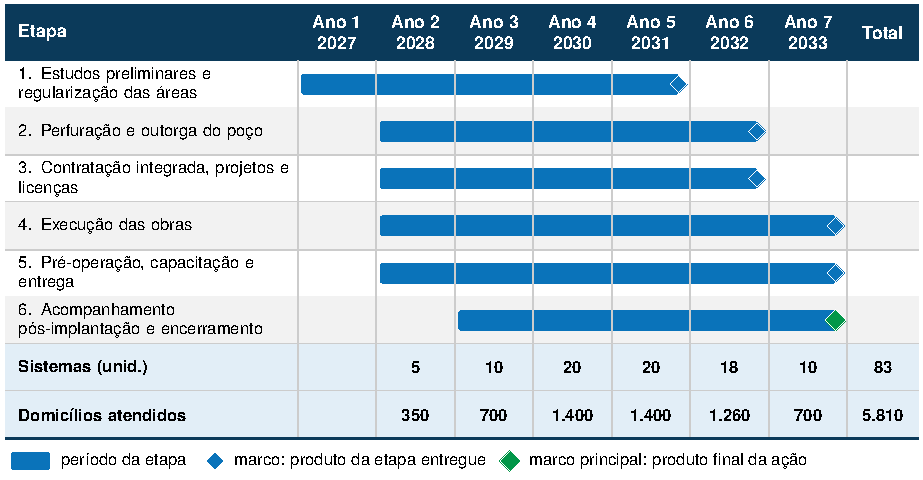
\includegraphics[width=15.64cm]{figuras/g-crono-3223.pdf}
  \fonteMOP{Fonte: IAT (2026), com quantidades da planilha PSH\_CUSTO\_Consolidada (PARANÁ, 2026).}
  % Texto alternativo: Cronograma anual de 2027 a 2033 com as etapas e as quantidades a entregar da implantação dos sistemas coletivos de abastecimento de água.
\end{figure}

\phantomsection
\addcontentsline{toc}{subsection}{9. Interfaces e dependências}
\subsection*{9. Interfaces e dependências}

A ação depende da entidade gestora pactuada, do diagnóstico das comunidades, da supervisão das obras e dos instrumentos de gestão de recursos hídricos do Programa, como a outorga, o SIGARH e os dados de águas subterrâneas. Fornece ao esgotamento sanitário as comunidades atendidas com água, aos modelos de gestão os sistemas concluídos para entrega e à UGP o número de pessoas atendidas para o indicador do componente (Figura~\ref{interf-3223}).

\begin{figure}[H]
  \centering
  \caption{Interfaces e dependências da implantação dos sistemas coletivos de abastecimento de água}\label{interf-3223}
  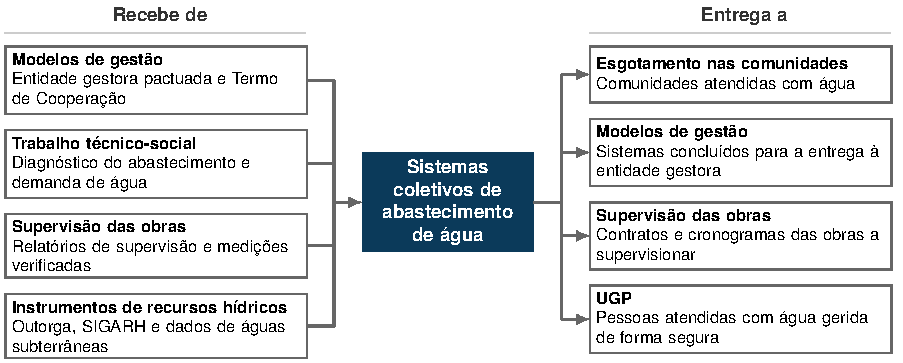
\includegraphics[width=15.30cm]{figuras/g-interf-3223.pdf}
  \fonteMOP{Fonte: IAT (2026).}
  % Texto alternativo: Diagrama das interfaces da implantação dos sistemas coletivos de abastecimento de água: insumos recebidos de outras partes do Programa e produtos entregues a elas.
\end{figure}

\phantomsection
\addcontentsline{toc}{subsection}{10. Documentos complementares}
\subsection*{10. Documentos complementares}

\begin{itemize}
  \item Termo de Referência e edital da contratação integrada de projetos e obras (a elaborar);
  \item Plano de Operação e Manutenção dos sistemas (a elaborar);
  \item Portaria GM/MS nº~888/2021, que altera o Anexo XX da Portaria de Consolidação GM/MS nº~5/2017 (padrão de potabilidade da água para consumo humano);
  \item Normas da Associação Brasileira de Normas Técnicas (ABNT) NBR 12212:2017 e NBR 12244:2006 (projeto e construção de poço tubular) e demais normas ABNT de projeto de sistemas de abastecimento de água;
  \item Lei nº~9.433/1997 e Lei Estadual nº~12.726/1999 (outorga de direito de uso de recursos hídricos) e normas de licenciamento ambiental do IAT;
  \item Caderno AQ e Caderno AS;
  \item Notas técnicas de origem (IAT, 2026a; IAT, 2026b).
\end{itemize}
